%%%%%%%%%%%%%%%%%%%%%%%%%%%%%%%%%%%%%%%%%%%%%%%%%%%%%%%%%%%%%%%%%%%%%%
% Overleaf (WriteLaTeX) Example: Molecular Chemistry Presentation
%
% Source: http://www.overleaf.com
%
% In these slides we show how Overleaf can be used with standard 
% chemistry packages to easily create professional presentations.
% 
% Feel free to distribute this example, but please keep the referral
% to overleaf.com
% 
%%%%%%%%%%%%%%%%%%%%%%%%%%%%%%%%%%%%%%%%%%%%%%%%%%%%%%%%%%%%%%%%%%%%%%

\documentclass{beamer}

\mode<presentation>
{
  \usetheme{Madrid}       % or try default, Darmstadt, Warsaw, ...
  \usecolortheme{default} % or try albatross, beaver, crane, ...
  \usefonttheme{default}    % or try default, structurebold, ...
  \setbeamertemplate{navigation symbols}{}
  \setbeamertemplate{caption}[numbered]
} 

\usepackage[english]{babel}
\usepackage[utf8x]{inputenc}
\usepackage{chemfig}
\usepackage[version=3]{mhchem}

\usepackage{hyperref}
  \hypersetup{colorlinks=true}
  \hypersetup{urlcolor=blue}
  \hypersetup{linkcolor = .}
\usepackage{xcolor}
\usepackage{siunitx}
  \sisetup{separate-uncertainty = true}
\usepackage{physics}
\usepackage[font=small,labelfont=bf]{caption}
\usepackage{subcaption}
\usepackage[en-GB]{datetime2}
\usepackage{overpic}
\usepackage{feynmp}
\DeclareGraphicsRule{*}{mps}{*}{}

\usepackage{scalerel}
\newcommand{\mylbrace}[2]{\vspace{#2pt}\hspace{6pt}\scaleleftright[\dimexpr5pt+#1\dimexpr0.06pt]{\lbrace}{\rule[\dimexpr2pt-#1\dimexpr0.5pt]{-4pt}{#1pt}}{.}}
\newcommand{\myrbrace}[2]{\vspace{#2pt}\scaleleftright[\dimexpr5pt+#1\dimexpr0.06pt]{.}{\rule[\dimexpr2pt-#1\dimexpr0.5pt]{-4pt}{#1pt}}{\rbrace}\hspace{6pt}}

% Here's where the presentation starts, with the info for the title slide
\title[BESIII Oxford]{BESIII Oxford Group Meeting}
\author{Martin Tat}
\institute{Oxford LHCb}
\date{27th May 2021}

\titlegraphic{
\includegraphics[width = 5cm, height = 3.8cm]{lhcb.jpg}\hspace{1cm}~%
              
\includegraphics[width = 5cm, height = 3.8cm]{bes3.jpg}}

\begin{document}

\begin{frame}
  \titlepage
\end{frame}

% These three lines create an automatically generated table of contents.
%\begin{frame}{Outline}
%  \tableofcontents
%\end{frame}

\section{Intorduction}
\begin{frame}{Introduction}
  \begin{itemize}
    \setlength\itemsep{2em}
    \item{$K_SKK$ double tag yields for $\delta_D^{K\pi}$ measurement}
    \item{Previously:}
    \begin{enumerate}
      \item{Selected $K_{S, L}KK$ events tagged with $K\pi$, $K\pi\pi^0$, $K\pi\pi\pi$ (and $Ke\nu$)}
      \item{Bin migration matrix and bin efficiencies from MC}
    \end{enumerate}
    \item{Today: Need help with peaking background subtraction}
  \end{itemize}
\end{frame}

\section{Fully reconstructed double tags}
\begin{frame}{Fully reconstructed double tags}
  \begin{itemize}
    \setlength\itemsep{2em}
    \item{$K_SKK$ vs $K\pi$, $K\pi\pi^0$, $K\pi\pi\pi$}
    \item{Count number of background events inside S from inclusive $D^0\bar{D^0}$ MC}
  \end{itemize}
  \begin{figure}
    \centering
    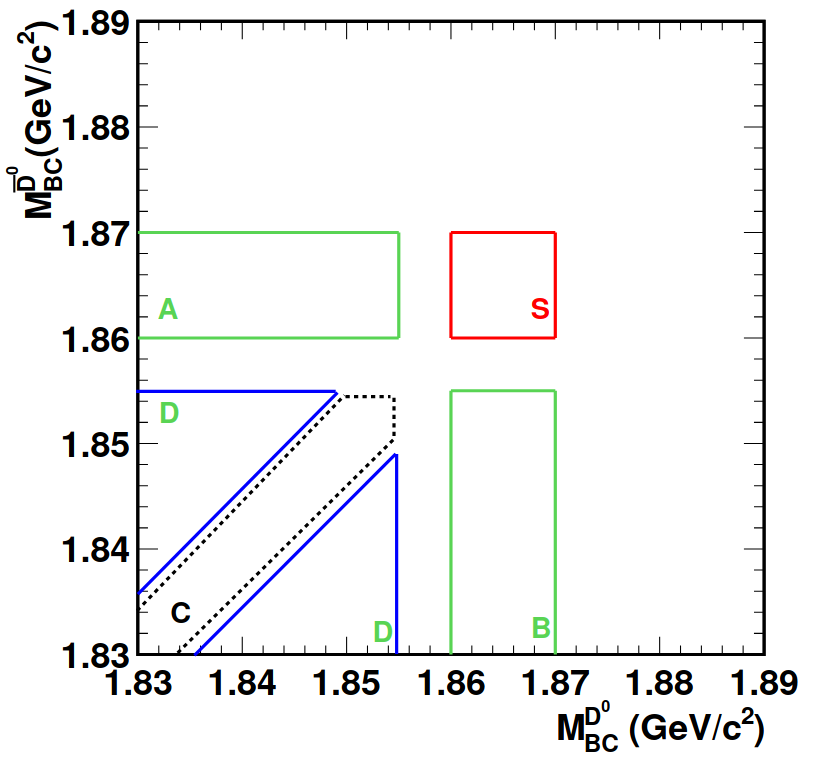
\includegraphics[width=0.40\textwidth]{MBC2D.png}
  \end{figure}
\end{frame}

\begin{frame}{$K\pi$ backgrounds}
  \begin{itemize}
    \item{Total data yield: $321.5$}
    \item{Scale with MC luminosity: $6912.3$}
  \end{itemize}
  \vspace{0.5cm}
  \centering
  \def\arraystretch{1.2}%
  \begin{tabular}{c|ccccc}
    Background              & Total  & Bin $1$ & Bin $2$ & Bin $-1$ & Bin $-2$ \\
    \hline
    $K_SKK\to KK\pi\pi$     & $10$   & $2$     & $1$     & $6$      & $1$ \\
    $K_SKK\to K_LKK$        & $5$    & $2$     & $0$     & $3$      & $0$ \\
    Other                   & $4$    & $0$     & $0$     & $2$      & $2$ \\
    \hline
  \end{tabular}
  \vspace{0.5cm}
  \begin{itemize}
    \item{How does $K_L\to K_S$ swap happen...?}
    \item{Can the MC be trusted?}
  \end{itemize}
\end{frame}

\begin{frame}{$K\pi\pi^0$ backgrounds}
  \begin{itemize}
    \item{Total data yield: $584.5$}
    \item{Scale with MC luminosity: $12742.1$}
  \end{itemize}
  \vspace{0.5cm}
  \centering
  \def\arraystretch{1.2}%
  \begin{tabular}{c|ccccc}
    Background                    & Total  & Bin $1$ & Bin $2$ & Bin $-1$ & Bin $-2$ \\
    \hline
    $K_SKK\to KK\pi\pi$           & $16$   & $9$     & $1$     & $5$      & $1$ \\
    $K\pi\to K\mu\nu_\mu$         & $8$    & $1$     & $2$     & $2$      & $3$ \\
    $K_SKK\to K_LKK$              & $8$    & $2$     & $0$     & $6$      & $0$ \\
    $K\pi\pi^0\to K\pi\pi^0\pi^0$ & $6$    & $2$     & $2$     & $1$      & $1$ \\
    $K\pi\to KK$                  & $4$    & $0$     & $3$     & $0$      & $1$ \\
    $K\pi\to Ke\nu_e$             & $3$    & $0$     & $2$     & $0$      & $1$ \\
    Other                         & $14$   & $0$     & $11$    & $0$      & $3$ \\
    \hline
  \end{tabular}
  \vspace{0.5cm}
\end{frame}

\begin{frame}{$K\pi\pi\pi$ backgrounds}
  \begin{itemize}
    \item{Total data yield: $399.6$}
    \item{Scale with MC luminosity: $8711.3$}
  \end{itemize}
  \vspace{0.5cm}
  \centering
  \def\arraystretch{1.2}%
  \begin{tabular}{c|ccccc}
    Background                      & Total  & Bin $1$ & Bin $2$ & Bin $-1$ & Bin $-2$ \\
    \hline
    $K\pi\pi\pi\to K_SK^+\pi^-$     & $43$   & $3$     & $21$    & $1$      & $18$ \\
    $K_SKK\to K_LKK$                & $9$    & $1$     & $0$     & $8$      & $0$ \\
    $K_SKK\to KK\pi\pi$             & $9$    & $4$     & $1$     & $3$      & $1$ \\
    $K\pi\pi\pi\to K\pi\pi^0\pi\pi$ & $6$    & $0$     & $1$     & $2$      & $3$ \\
    Other                           & $13$   & $2$     & $5$     & $2$      & $4$ \\
    \hline
  \end{tabular}
  \vspace{0.5cm}
\end{frame}

\section{Next steps}
\begin{frame}{Next steps}
  \begin{itemize}
    \setlength\itemsep{2em}
    \item{DCS correction?}
    \item{Finalize the final yields}
    \item{Propagate the errors}
  \end{itemize}
\end{frame}

\end{document}
